%\documentclass[draft]{beamer}
\documentclass{beamer}

\mode<presentation>
{
  %\usetheme[secheader]{Boadilla}
  \usetheme{default}
}

\usepackage{calc}
%\usepackage{multimedia}
\usepackage{movie15}

\usepackage[english]{babel}

\usepackage[latin1]{inputenc}

\usepackage{times}
\usepackage[T1]{fontenc}

\newcommand{\figref}[1]{\begin{flushright}{\tiny #1 }\end{flushright}}

\title[FA Characterization]{Automatic Characterization of Focal Adhesions in TIRF Microscopy Images}

\author[] % (optional, use only with lots of authors)
{Matthew E. Berginski}
\institute[]{University of North Carolina at Chapel Hill}
% - Use the \inst{?} command only if the authors have different
%   affiliation.
  
\date[9/8/2008 Hahn Lab Meeting]{7/29/2009 Hahn Lab Meeting}


\usecolortheme[RGB={2,91,173}]{structure}

\begin{document}

\begin{frame}
	\titlepage
	\includegraphics[width=0.25\textwidth]{ghost}
\end{frame}

\section{Introduction}

\begin{frame}
	\frametitle{Focal What?}
	\begin{columns} 
		\column{.5\textwidth} 
		\begin{itemize}
		\item Points of contact between the substrate and cells
		\item Consist of dozens of dynamically recruited proteins
		\item Important in understanding how cells navigate and sample the environment
		\end{itemize}		

		\column{.5\textwidth}
		\only<1>{
		\begin{center}
		\begin{figure}[htbp]
		\includegraphics[width=5cm]{figures/intro/adhesion_overview}	
		\end{figure}
		\end{center}
		\figref{E. Zamir and B. Geiger. JCS, 114(20):3583-3590, 2001.}
		}
		\only<2>{
		\begin{center}
		\begin{figure}[htbp]
		\includegraphics[width=5cm]{figures/intro/Pax_closeup}
		\end{figure}
		\end{center}
		\figref{E. Zamir and B. Geiger. JCS, 114(20):3583-3590, 2001.}		
		}
	\end{columns} 
\end{frame}

\begin{frame}
	\frametitle{Paxillin Info/Example Movie}
	\begin{columns}
		\column{0.5\textwidth}
		\begin{itemize}
		\item Paxillin - adhesion scaffolding protein
		\item Recruited to adhesions early, remains associated
		\item Data consists of time lapse images of GFP-labeled Paxillin in 3T3 fibroblasts
		\end{itemize}
		\column{0.5\textwidth}
		\begin{center}
		\begin{figure}[htbp]
		\includegraphics[width=5cm]{figures/intro/sample_original_data_w_eric}
		\end{figure}
		\end{center}
	\end{columns}
\end{frame}

\begin{frame}
  \frametitle{Outline}
  \tableofcontents
\end{frame}

\section[Finding/Tracking]{Finding/Tracking Adhesions}

\subsection{Identifying Focal Adhesions}
\begin{frame}
	\frametitle{Identification Overview}
	\begin{columns}
	\column{0.5\textwidth}
	\begin{itemize}
	\item Prior Methods
	\item Multistage process
		\begin{itemize}
		\item Finding Adhesions
		\item Tracking Adhesions
		\item Visualization
		\end{itemize}
	\end{itemize}
	\column{0.5\textwidth}
	\includegraphics[width=\textwidth]{figures/finding/ident_overview}
	\end{columns}
\end{frame}

\begin{frame}
	\frametitle{Prior Methods}
	\begin{center}
	\includegraphics[width=0.8\textwidth]{figures/finding/prior}
	\end{center}
	\figref{D. Webb, et al. NCB, 6(2):154-161, 2004.}
\end{frame}

\begin{frame}
	\frametitle{Determining Adhesion Pixels}
	 \begin{itemize}
	 \item Technique adapted from E. Zamir, et al. JCS, 112(11):1655-1669, 1999.
	 \item High-pass image filter applied
	 \item Threshold used to select pixels
	 \end{itemize}
	 \bigskip
	 \begin{center}
	 \includegraphics[width=0.95\textwidth]{figures/finding/pixel_id}
	 \end{center}

\end{frame}

\begin{frame}
	\frametitle{Threshold Variation}
	\begin{figure}
		\includegraphics[width=0.2\textwidth]{figures/finding/thresh_examples/00.png}
		\includegraphics[width=0.2\textwidth]{figures/finding/thresh_examples/01.png}
		\includegraphics[width=0.2\textwidth]{figures/finding/thresh_examples/02.png}
		\includegraphics[width=0.2\textwidth]{figures/finding/thresh_examples/03.png}
		\\
		\includegraphics[width=0.2\textwidth]{figures/finding/thresh_examples/04.png}
		\includegraphics[width=0.2\textwidth]{figures/finding/thresh_examples/05.png}
		\includegraphics[width=0.2\textwidth]{figures/finding/thresh_examples/06.png}
		\includegraphics[width=0.2\textwidth]{figures/finding/thresh_examples/07.png}
		\\
		\includegraphics[width=0.2\textwidth]{figures/finding/thresh_examples/08.png}
		\includegraphics[width=0.2\textwidth]{figures/finding/thresh_examples/09.png}
		\includegraphics[width=0.2\textwidth]{figures/finding/thresh_examples/10.png}
	\end{figure}
\end{frame}

\begin{frame}
	\frametitle{Assigning Pixels to Adhesions}
	\begin{columns}
		\column{0.5\textwidth}
		\begin{itemize}
		\item Technique adapted from E. Zamir, et al. JCS, 112(11):1655-1669, 1999.
		\item High-passed pixel values are sorted, then added singly
		\item Each added pixel, joins a current adhesion or starts a new adhesion
		\item Merging limited to small adhesions
		\end{itemize}
		\column{0.5\textwidth}
		\includegraphics[width=\textwidth]{figures/finding/ad_pixels_example}
	\end{columns}
\end{frame}

%\subsection{Tracking the Adhesions}
%
%\begin{frame}
%	\frametitle{Tracking System}
%	\begin{columns}
%		\column{0.5\textwidth}
%		\begin{itemize}
%		\item Based on a birth-death model of adhesion life
%		\item Tracking is based on adhesion centroid position and pixel overlap with adhesions in next frame
%		\end{itemize}
%		\column{0.5\textwidth}
%		\begin{center}
%		\includegraphics[height=0.75\textheight]{figures/finding/flow_charts/fa_workflow.pdf}
%		\end{center}
%	\end{columns}
%\end{frame}
%
%\begin{frame}
%	\frametitle{Tracking System - Initialization}
%	\begin{columns}
%		\column{0.5\textwidth}
%		\includegraphics[width=\textwidth]{figures/finding/all_highlight_sample}
%		\column{0.5\textwidth}
%		\begin{center}
%		\includegraphics[height=0.75\textheight]{figures/finding/flow_charts/highlights/fa_workflow_init.pdf}
%		\end{center}
%	\end{columns}
%\end{frame}
%
%\begin{frame}
%	\frametitle{Tracking System - Tracking Live Adhesions}
%	\begin{columns}
%		\column{0.5\textwidth}
%		\begin{center}
%		 \includegraphics{figures/finding/tracking_images/live_track_1}
%		 \end{center}
%		\column{0.5\textwidth}
%		\begin{center}
%		\includegraphics[height=0.75\textheight]{figures/finding/flow_charts/highlights/fa_workflow_live.pdf}
%		\end{center}
%	\end{columns}
%\end{frame}
%
%\begin{frame}
%	\frametitle{Tracking System - Merge/Death}
%	\begin{columns}
%		\column{0.5\textwidth}
%		\begin{figure}
%		\includegraphics[width=\textwidth]{figures/finding/tracking_images/death_example_1}
%		\end{figure}
%		\begin{figure}
%		\includegraphics[width=\textwidth]{figures/finding/tracking_images/death_example_2}
%		\end{figure}
%		\column{0.5\textwidth}
%		\begin{center}
%		\includegraphics[height=0.75\textheight]{figures/finding/flow_charts/highlights/fa_workflow_md.pdf}
%		\end{center}
%	\end{columns}
%\end{frame}
%
%\begin{frame}
%	\frametitle{Tracking System - Start New Lineages}
%	\begin{columns}
%		\column{0.5\textwidth}
%		\begin{figure}
%		\includegraphics[width=\textwidth]{figures/finding/tracking_images/birth_example_1}
%		\end{figure}
%		\begin{figure}
%		\includegraphics[width=\textwidth]{figures/finding/tracking_images/birth_example_2}
%		\end{figure}		
%		\column{0.5\textwidth}
%		\begin{center}
%		\includegraphics[height=0.75\textheight]{figures/finding/flow_charts/highlights/fa_workflow_new.pdf}
%		\end{center}
%	\end{columns}
%\end{frame}

\subsection{Visualizing the Results}

\begin{frame}
	\frametitle{Visualizing Single Adhesions}
	\begin{center}
	\includegraphics[height=0.75\textheight]{figures/finding/montage_00004}
	\end{center}
\end{frame}

\begin{frame}
	\frametitle{Tracking Example Movie - Unique Colors}
	\begin{center}
	\includegraphics[width=10.88cm]{figures/finding/orig_track_sample}
	\end{center}
\end{frame}

\begin{frame}
	\frametitle{Tracking Example Movie - Birth Time Colors}
	\begin{center}
	\includegraphics[width=10.88cm]{figures/finding/time_track_sample}
	\end{center}
\end{frame}

\section[Properties]{Adhesion Properties}

\begin{frame}
	\frametitle{Properties Overview}
	\begin{itemize}
	\item General Adhesion Lifecycle properties:
		\begin{itemize}
		\item Adhesion birth and death locations
		\item Adhesion lifetimes
		\end{itemize}
	\item Assembly and Disassembly Rates
	\end{itemize}
\end{frame}

\begin{frame}
	\frametitle{General Dynamics Properties}
	\only<1>{
		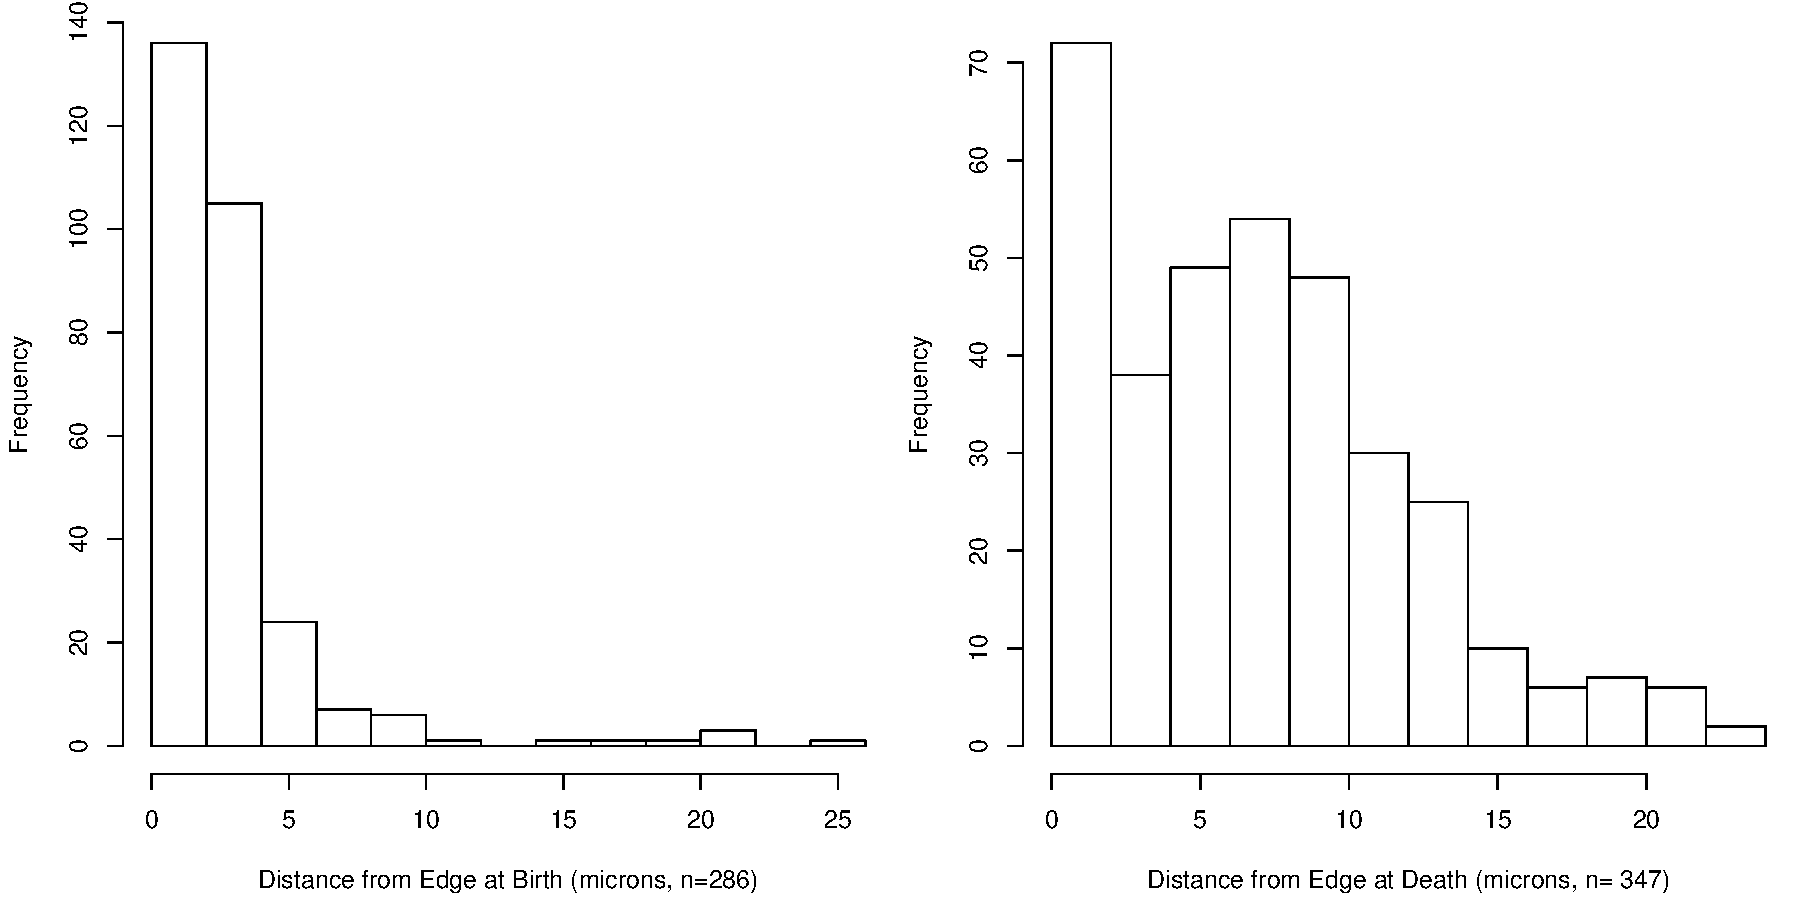
\includegraphics[width=\textwidth]{figures/analysis/dist_hists}
	}
	\only<2>{
		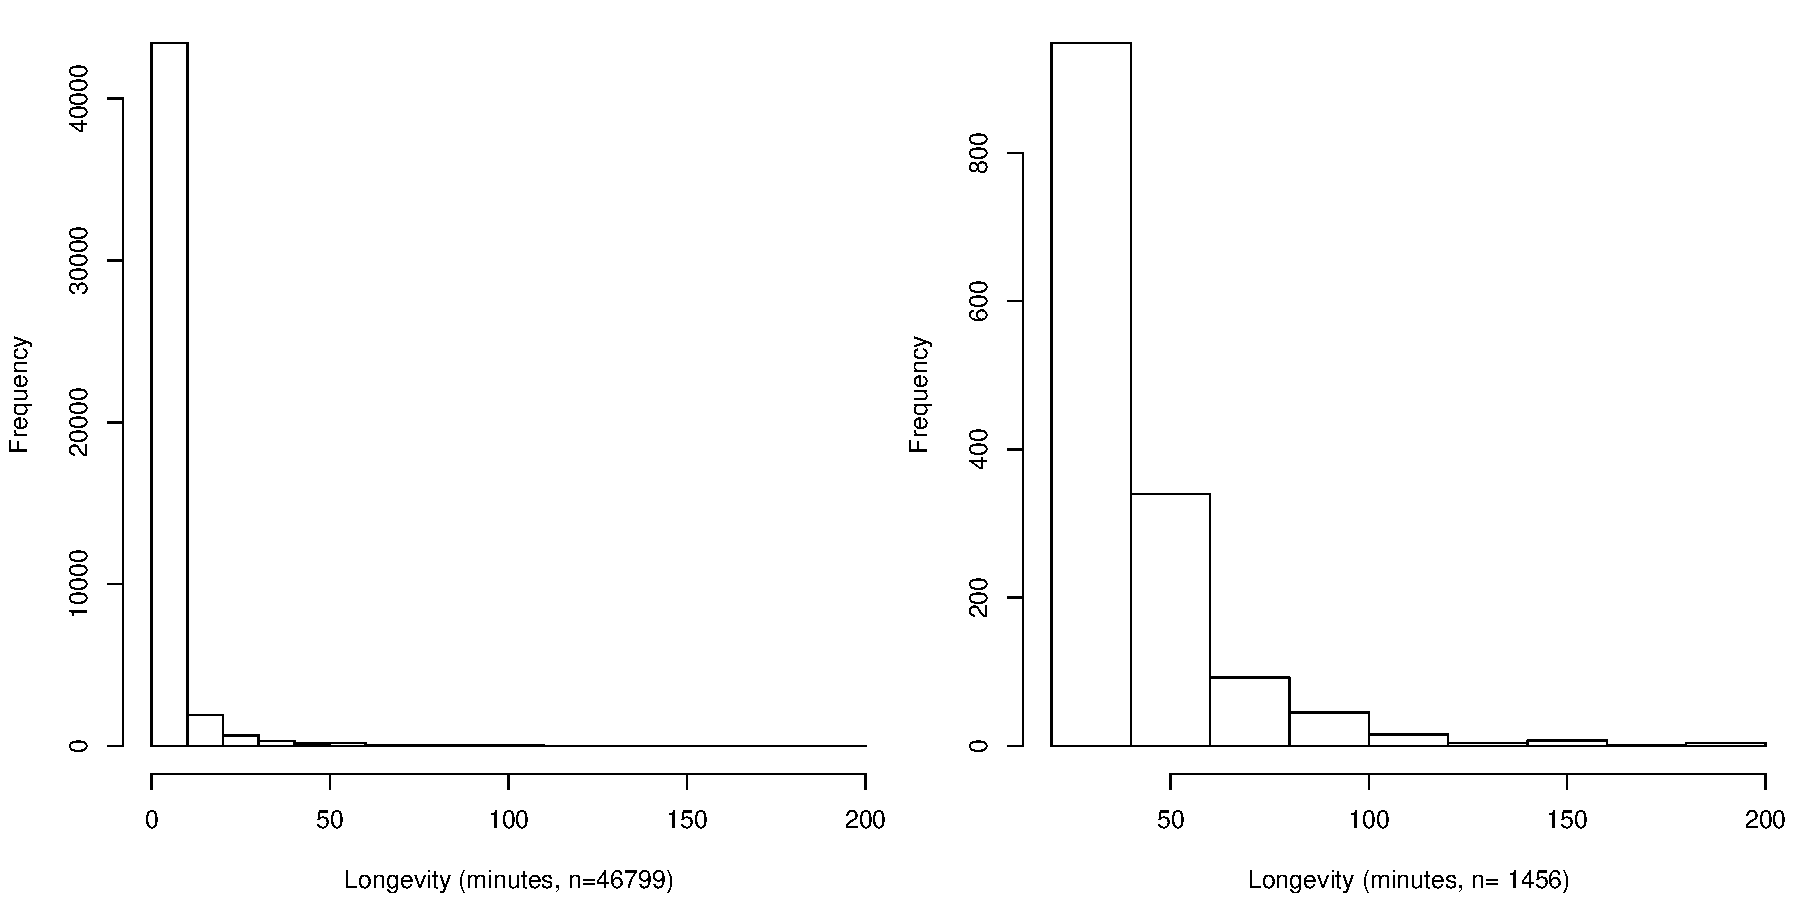
\includegraphics[width=\textwidth]{figures/analysis/longev_hists}
	}
\end{frame}

\begin{frame}
	\frametitle{Single Adhesion Assembly and Disassembly Rates}
	\only<1> {
	\begin{center}
	\includegraphics[height=0.75\textheight]{figures/analysis/montage_01154}
	\end{center}
	}
	\only<2>{
	\begin{center}
	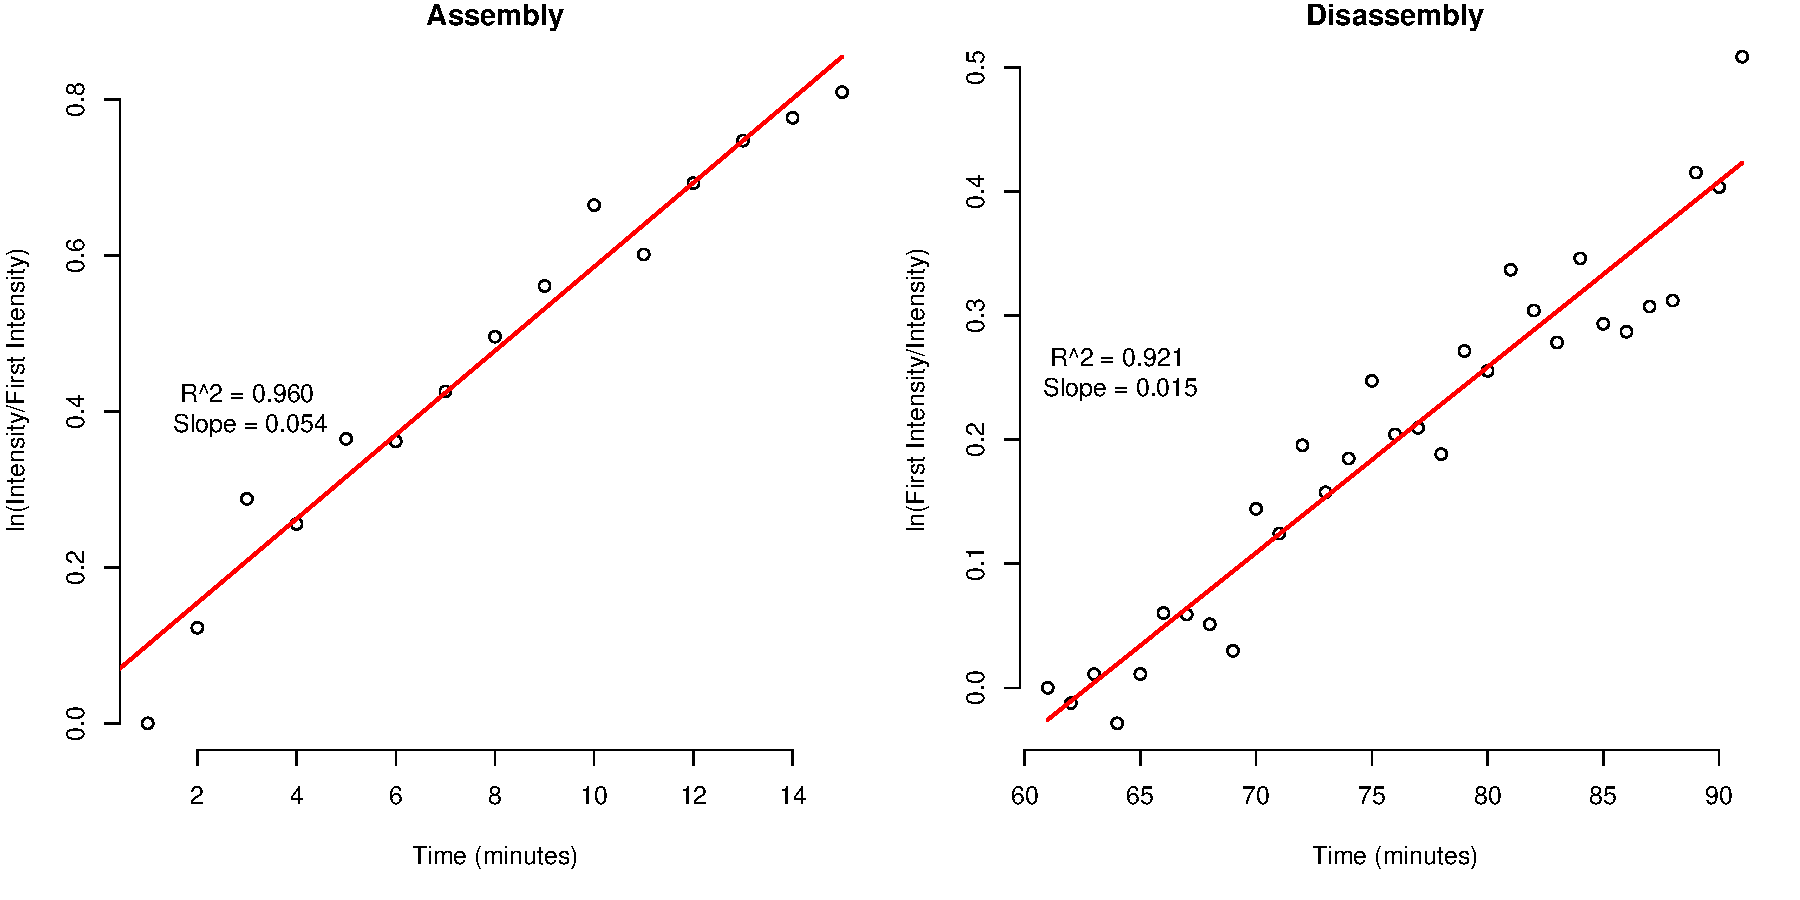
\includegraphics[width=\textwidth]{figures/analysis/accum_decay_1154}
	\end{center}
	}
\end{frame}

\begin{frame}
	\frametitle{Rate Fit Qualities}
	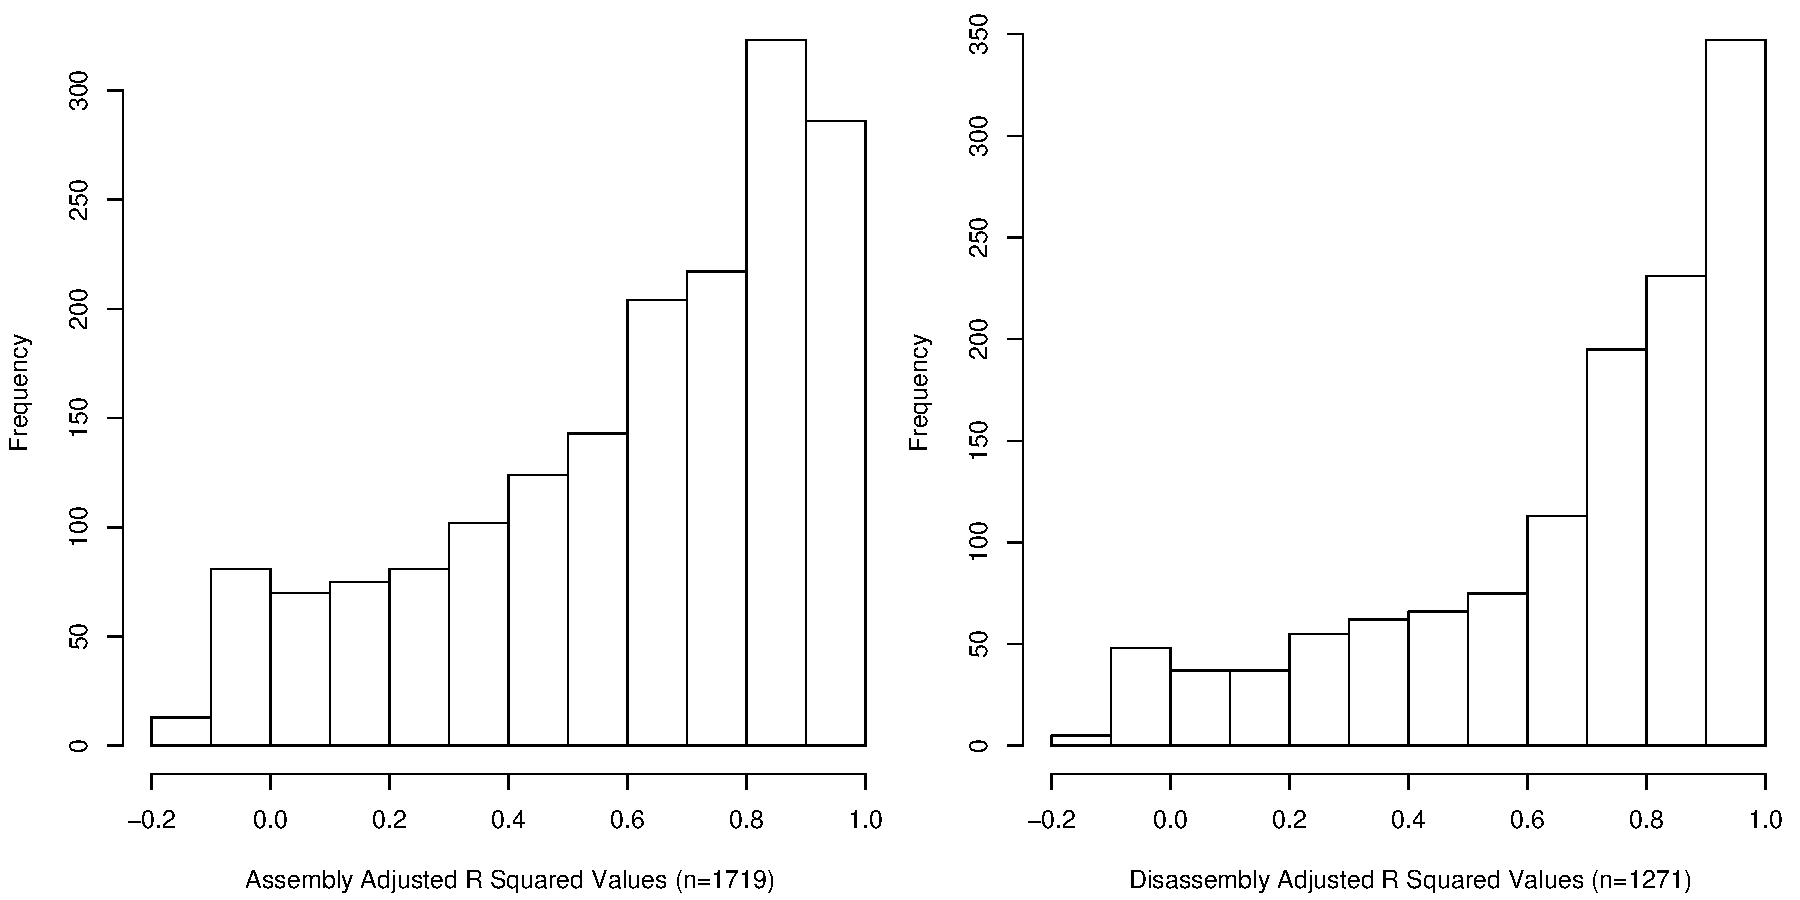
\includegraphics[width=\textwidth]{figures/analysis/R_sq_hist_all}
\end{frame}

\begin{frame}
	\frametitle{Overall Rate Summary}
	\begin{center}
	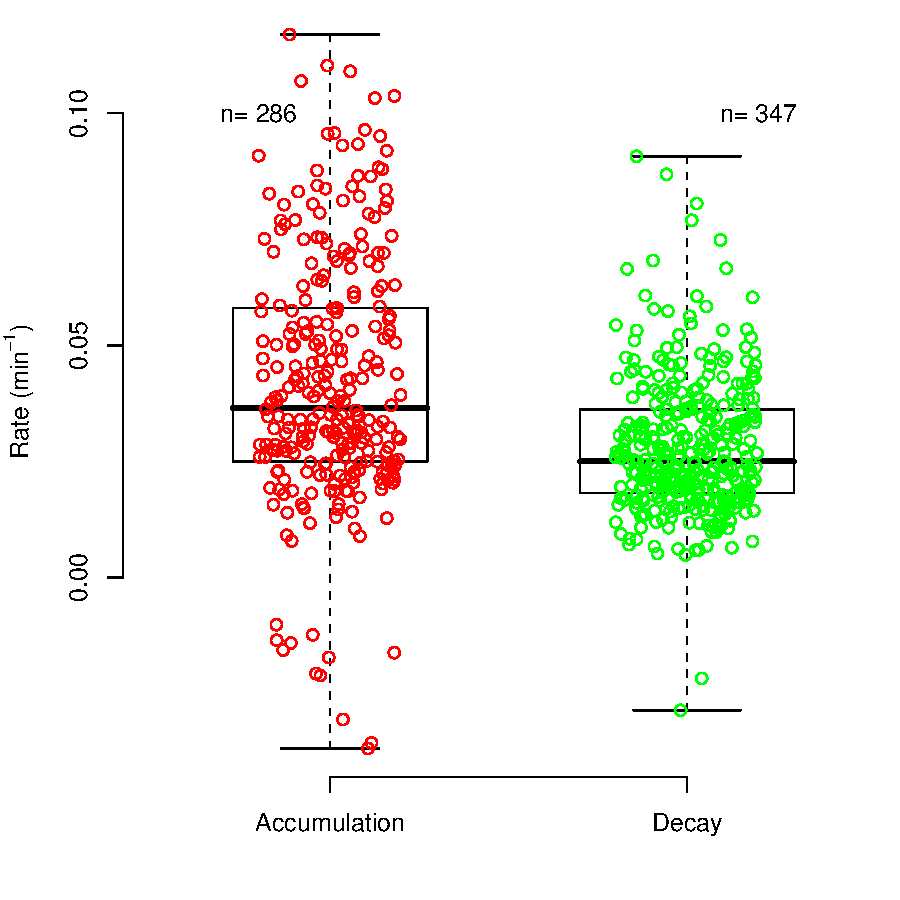
\includegraphics[height=0.85\textheight]{figures/analysis/accum_decay_single_colors}
	\end{center}
\end{frame}

\section[]{Conclusions}

\begin{frame}
	\frametitle{Conclusions/Future Work}
	\begin{columns}
	\column{0.5\textwidth}
		\begin{itemize}
		\item System for extracting properties for labeled adhesions:
			\begin{itemize}
			\item Finding
			\item Tracking
			\item Visualization
			\item Properties
			\end{itemize}
		\item Future Work:
			\begin{itemize}
			\item integration of biosensor data
			\end{itemize}
		\end{itemize}
	\column{0.5\textwidth}
		\begin{center}
		\includegraphics[height=0.4\textheight]{figures/finding/ident_overview}
		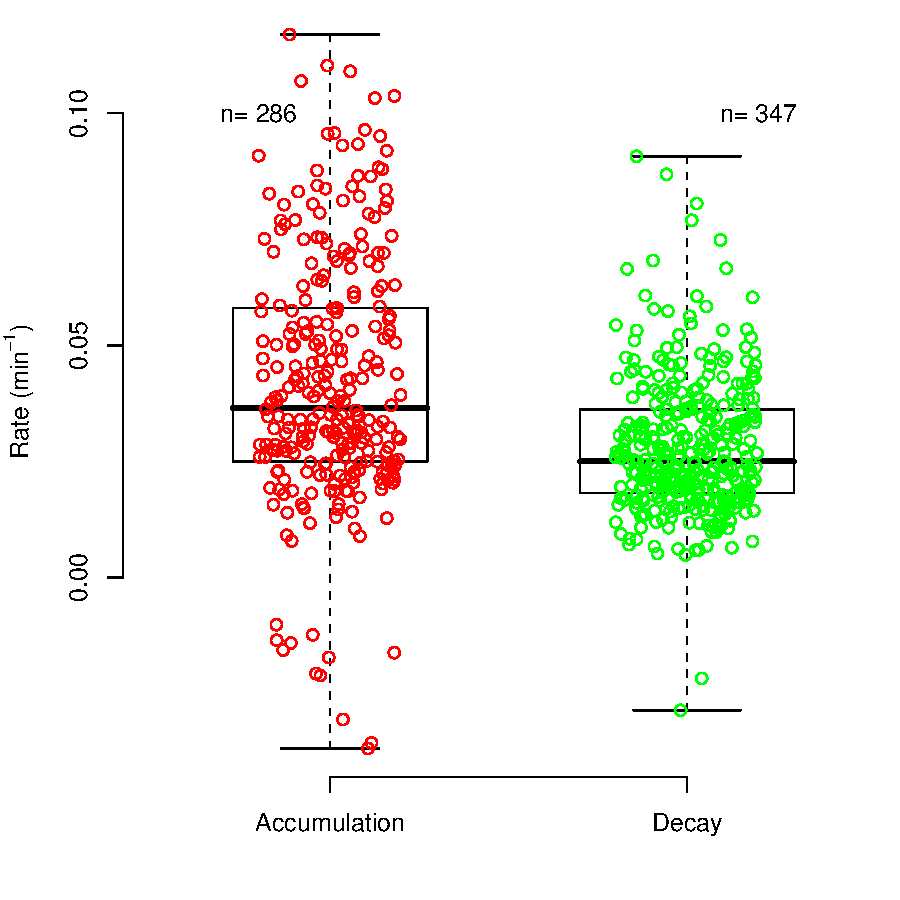
\includegraphics[height=0.4\textheight]{figures/analysis/accum_decay_single_colors}
		\end{center}
	\end{columns}
\end{frame}

\begin{frame}
  \frametitle{Questions?}
\end{frame}

\end{document}
